\documentclass[a4paper, 10pt]{article}
\usepackage[utf8]{inputenc}
\usepackage[english,russian]{babel}
\usepackage{fancyhdr}
\usepackage{caption}
\usepackage[left=1.5cm,right=1.5cm,top=2cm,bottom=1.5cm,bindingoffset=0cm]{geometry}
\captionsetup{labelsep=period}
\pagestyle{fancy}
\usepackage{listings,longtable,amsmath,amsfonts,graphicx,tikz,tabularx}

\lstset{
    basicstyle=\footnotesize,
    breakatwhitespace=false,
    breaklines=true,
    extendedchars=true,
    keepspaces=true,
    keywordstyle=\bfseries,
    numbers=left,
    numbersep=3pt,
    numberstyle=\tiny,
    showspaces=false,
    showstringspaces=false,
    showtabs=false,
    stepnumber=1,
    stringstyle=\emph,
    tabsize=2
}
\usepackage[export]{adjustbox}
\usepackage{graphicx}
%\graphicspath{ {images/} }

\usepackage{rotating}
\usepackage{pdflscape}

\renewcommand{\headrulewidth}{0pt}
\fancyfoot[L] {\thepage\bf}
\fancyfoot[C] {}

\begin{document}
    \begin{titlepage}
        \begin{center}
            \large
            Университет ИТМО
            \vspace{3cm}


            Кафедра вычислительной техники
            \vspace{4cm}

            \textsc{ \textbf{Отчёт по лабораторной работе  № 2} \\ 
            по дисциплине: "Схемотехника ЭВМ"}\\Вариант №5\\[8mm]

            \bigskip
        \end{center}
        \vspace{3cm}

        \hfill\begin{flushright}
             Студенты:
             Куклина М.Д. \\
             Кириллова А.А.
             \vfill
             Преподаватель:
        \end{flushright}
        \vfill
        \vfill
        \vfill
        \vfill
        \vfill
        \begin{center}
            Санкт-Петербург \\2016 г.
        \end{center}
    \end{titlepage}
   \newpage
    \section*{Содержание}
        \begin{enumerate}
            \item Цели работы.
            \item RTL модель.
            \item Временные диаграммы.
            \item Листинг.
            \item Вывод.
        \end{enumerate}

    \section*{Цели работы}
        \begin{enumerate}
            \item Знакомство с принципами работы последовательных интерфейсов ввода/вывода: I2C, SPI, UART.
            \item Изучение основ разработки аппаратных контроллеров периферийных устройств.
            \item  Изучение основ работы с цифровыми датчиками.
        \end{enumerate} 

     \section*{RTL модель}
        \begin{figure}[ht]
            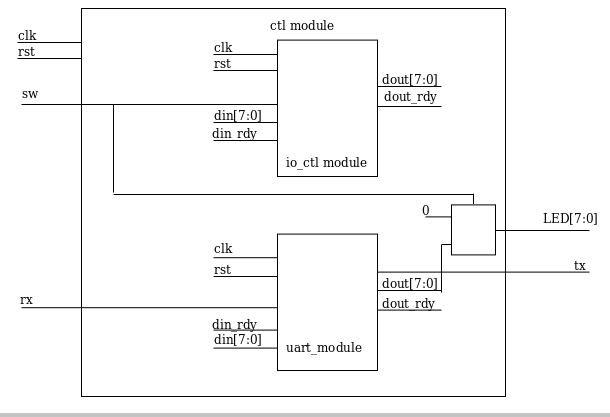
\includegraphics[scale=0.7]{../images/rtl_ctl.png}
        \end{figure}
        \begin{figure}[ht]
            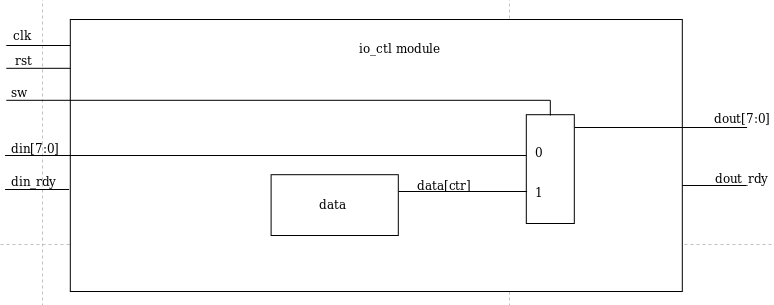
\includegraphics[scale=0.4]{../images/rtl_io.png}
        \end{figure}
        \begin{landscape}
            \begin{figure}[ht]
                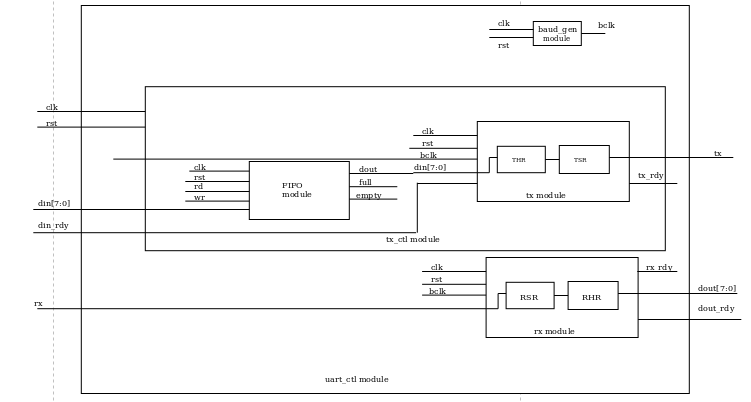
\includegraphics{../images/rtl_uart.png}
            \end{figure}
        \end{landscape}
     \section*{Временные диаграммы}
        \begin{figure}[h!]
            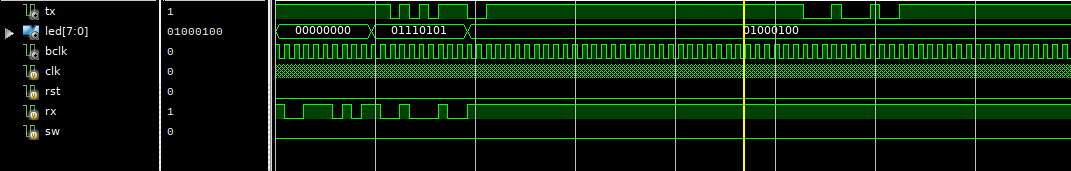
\includegraphics[scale=0.5]{../images/ctl_plot.png}
        \end{figure}
        \begin{figure}[h!]
            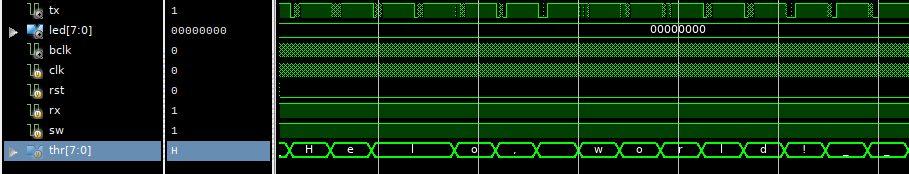
\includegraphics[scale=0.5]{../images/ctl_plot_send_mode.png}
        \end{figure}

     \section*{Листинг}
        \lstinputlisting[language=Verilog]{../src/ctl.v}
        \lstinputlisting[language=Verilog]{../src/io_ctl.v}
        \lstinputlisting[language=Verilog]{../src/uart_ctl.v}
        \lstinputlisting[language=Verilog]{../src/rx.v}
        \lstinputlisting[language=Verilog]{../src/tx_ctl.v}
        \lstinputlisting[language=Verilog]{../src/tx.v}
        \lstinputlisting[language=Verilog]{../src/fifo.v}
        \lstinputlisting[language=Verilog]{../src/baud_gen.v}

    \section*{Вывод}
        В ходы выполнения лабораторной работы были исследованы принципы работы
        последовательных интерфейсов I/O и в результате разработан универсальный
        асинхронный интерфейс UART.
\end{document}
